\documentclass[11pt,a4paper,oneside]{article}
\usepackage[utf8]{vietnam}
\newcommand{\contestname}{Pre Duyên Hải 2017}
\usepackage{olymp}
\usepackage[dvips]{graphicx}
\usepackage{color}
\usepackage{colortbl}
\usepackage{graphicx}
%\usepackage{expdlist}
%\usepackage{mfpic}
%\usepackage{comment}

% Treat all pictures as MPS (metapost) when using PDFLaTeX tool
%\ifx\pdftexversion\undefined
%\else
%  \DeclareGraphicsRule{*}{mps}{*}{}
%\fi

%\textsc{\renewcommand{\contestname}{
%}

% Copied from 'amstex.tex' \bmod declaration
\def\bdiv{\mskip-\medmuskip\mkern5mu\mathbin{\mathrm{div}}\mkern5mu\mskip-\medmuskip}
% End of copied text

\renewcommand{\t}{\texttt}

\begin{document}


% Tell LaTeX to make the title.
%\maketitle
% Tell LaTex to double space your text.
%\doublespacing
%\section{Topic 5}
\begin{problem}{Mua vé}{Standard Input}{Standard Output}{1 giây}{256}

Không chỉ đi thi NOI (National Olympiad in Informatics), Phễu còn được cho đi chơi khắp cả Singapore.
Singapore có N địa điểm vui chơi giải trí như Vivo City, Sentosa, Garena, Garden by The Bay, ...

\begin{figure}[h]
\centering
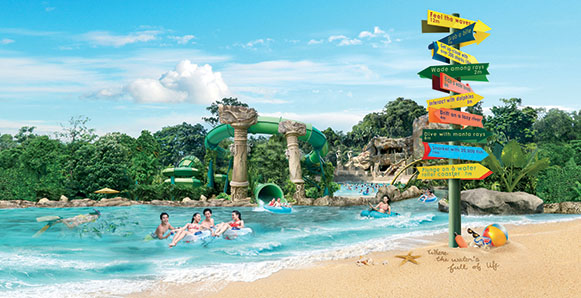
\includegraphics[width=0.75\textwidth]{sentosa}
\caption{Sentosa}
\end{figure}

\begin{figure}[h]
\centering
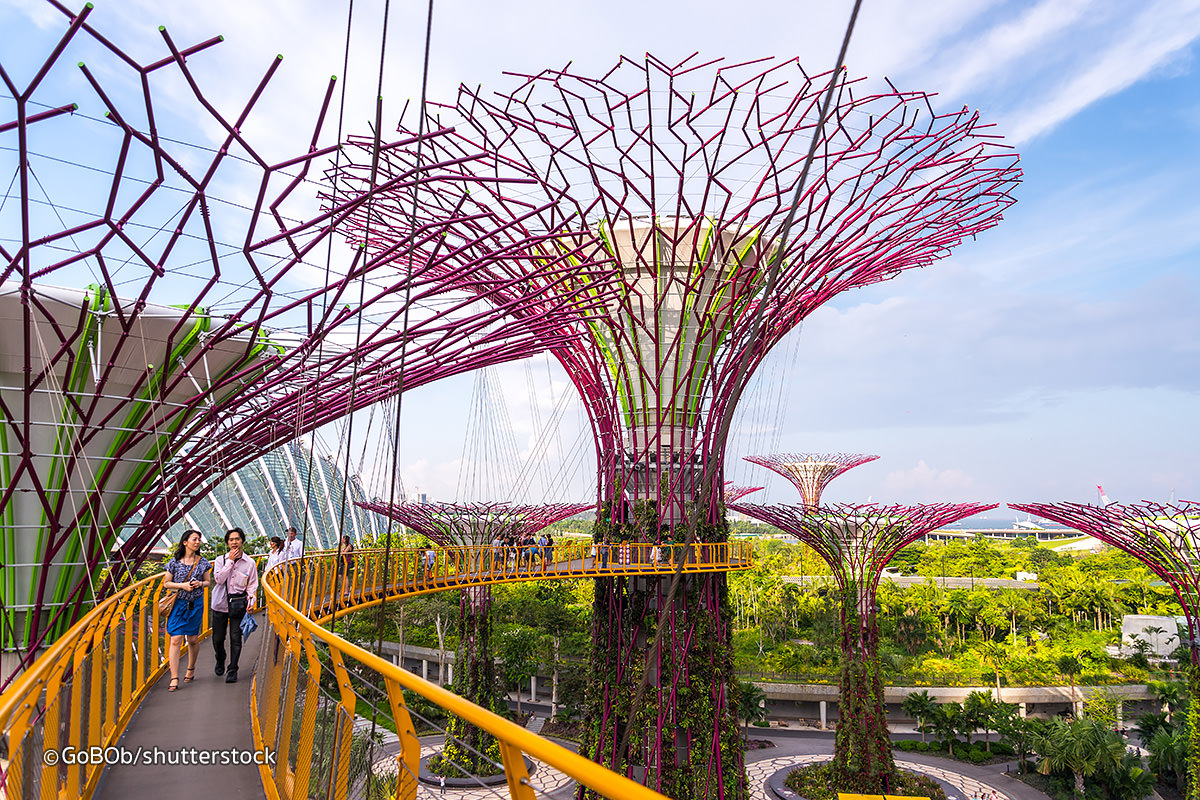
\includegraphics[width=0.75\textwidth]{gardens-by-the-bay-supertree-grove}
\caption{Garden by the Bay}
\end{figure}

Điều đáng lo ngại nhất là vé vào cửa. Đối với mỗi địa điểm thứ i, nếu Phễu lần đầu ghé thăm, sẽ được vào 
chơi miễn phí (tại Phễu béo), và từ lần thứ hai trở đi, giá vẽ sẽ tăng một lượng là $A_i$; nói cách khác,
lần đầu vào địa điểm i mất 0 đô, lần 2 mất $A_i$ đô, lần 3 mất $2 * A_i$ đô, lần 4 mất $3 * A_i$ đô, ...

\begin{figure}[h]
\centering
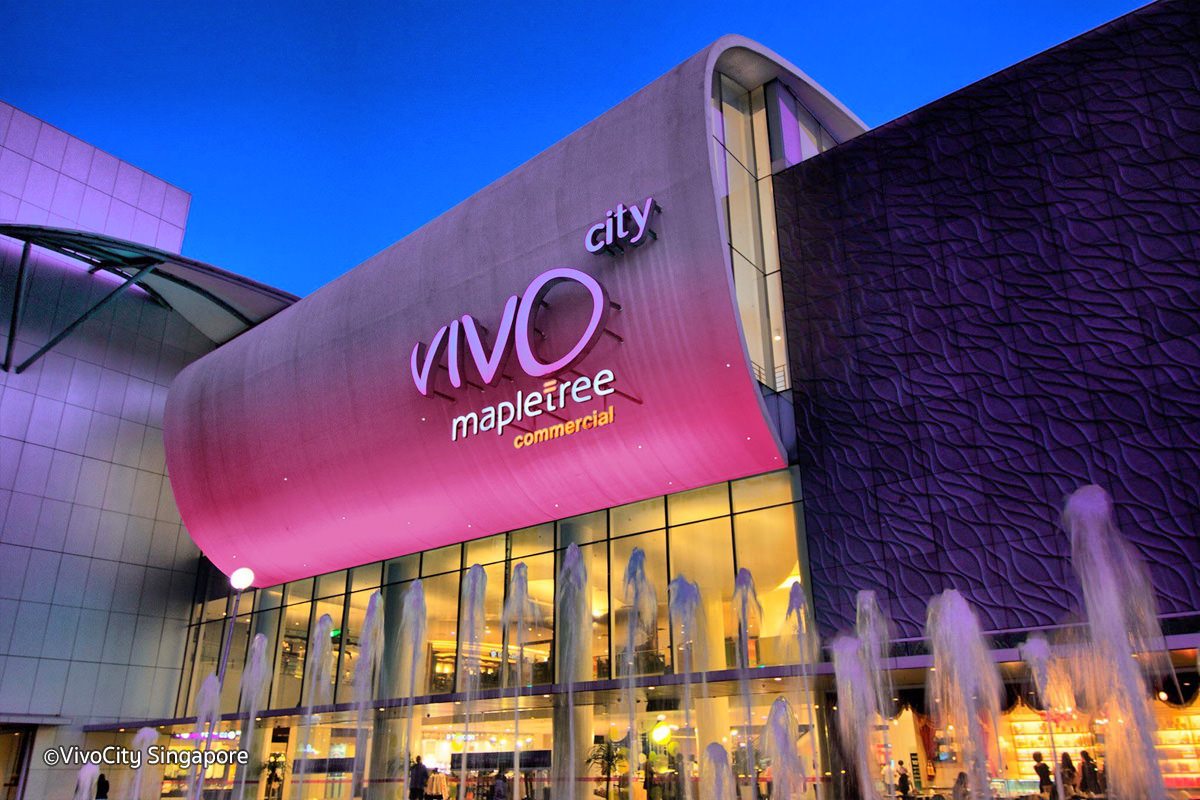
\includegraphics[width=0.75\textwidth]{VivoCity-Singapore}
\caption{Vivo City SG}
\end{figure}

Phễu muốn đi chơi X lần, đồng thời Phễu không ngại thăm quan một địa điểm nhiều lần.
 
Phễu sẽ phải đốt ít nhất bao nhiêu tiền sau X lần đi chơi?

\InputFile

\begin{itemize}
	\item Dòng đầu tiên ghi 2 số $N$ và $X$.
	\item Dòng tiếp theo ghi $N$ số $A_i$.
\end{itemize}

\OutputFile

\begin{itemize}
	\item In ra 1 số duy nhất là chi phí nhỏ nhất để mua vé.
\end{itemize}

\Constraints
\begin{itemize}
	\item $1 \le A_i \le 100$ (Để đảm bảo chi phí không quá $10^{18}$)
	\item Subtask 1 (10\% số điểm):
	\begin{itemize}
		\item $1 \le N \le 100$
		\item $1 \le X \le 500$
	\end{itemize}
	\item Subtask 2 (30\% số điểm):
	\begin{itemize}
		\item $1 \le N \le 10^5$
		\item $1 \le X \le 5 \times 10^5$
	\end{itemize}
	\item Subtask 3 (60\% số điểm):
	\begin{itemize}
		\item $1 \le N \le 10^5$
		\item $1 \le X \le 10^9$
	\end{itemize}
\end{itemize}

\Example

\begin{example}
\exmp{
3 5
1 2 3
}{
3 
}%
\end{example}

\vspace{.5cm}
Ta mua 2 vé loại 1, 2 vé loại 2 và 1 vé loại 3.

\begin{figure}[h]
\centering
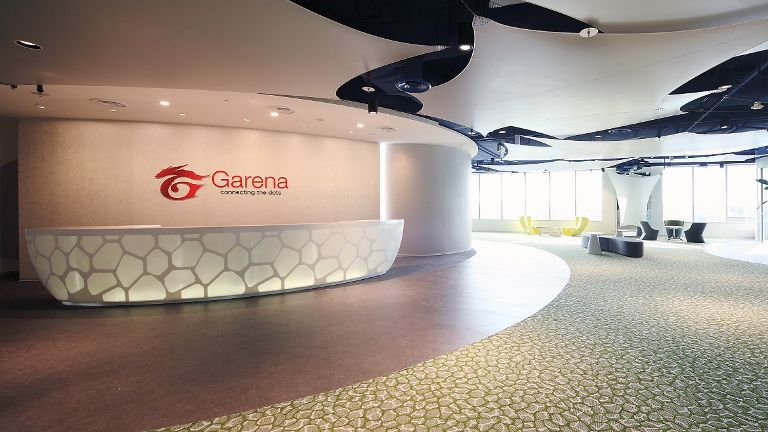
\includegraphics[width=0.75\textwidth]{garena-office-in-fusionopolis}
\caption{Garena HQ}
\end{figure}

\end{problem}

\end{document}
